\subsection{Multipliers}
\label{sec:implementation_multipliers}
\label{sec:implementation_multiplication}

While the simple arithmetic (addition, negation) of a point depends on its curve, algorithms for speeding up scalar
multiplication of points are often independent of the type of curve. For example, the Double-and-Add algorithm can be
applied to a point on any type of curve and -- regardless of the curve type -- result in the same performance improvement.
The same applies for the NAF and wNAF algorithms.

\begin{figure}[htb]
	\centering
	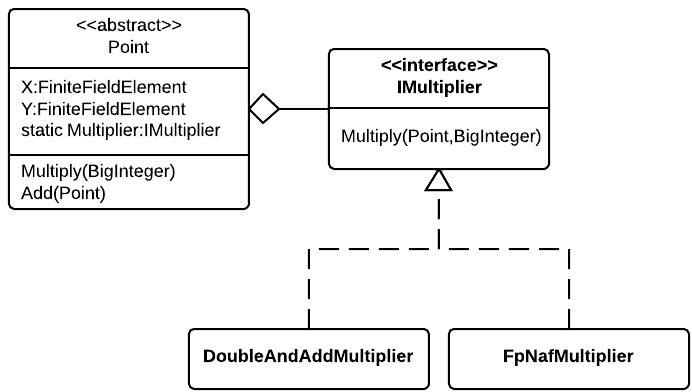
\includegraphics[width=0.7\textwidth]{implementation/multipliers}
	\caption{The relationship between points and multipliers. The multiplier is defined for all types of points, as it
		is set as a static property on the \texttt{Point} abstract class.}
\end{figure}

The possibility for changing a multiplier (and hence a multiplication algorithm) without having to change the code
performing the simple arithmetic both encourages such improvements, and enables performance comparisons of multiplication
algorithm candidates.

Some types of curves have specific methods for multiplication that are only applicable to that exact type of curve. For
example, Montgomery curves can take advantage of the \emph{Montgomery ladder} method, which significantly improves
performance.\cite{safecurves}

As such methods exist, setting a multiplier for \emph{all} points (no matter if they belong to Montgomery, Edwards, or
Weierstrass curves) does not seem a smart move. The design should be altered in future revisions to take this into account,
setting the multiplier on a per-curve-type basis.